\documentclass[twoside]{book}

% Packages required by doxygen
\usepackage{fixltx2e}
\usepackage{calc}
\usepackage{doxygen}
\usepackage[export]{adjustbox} % also loads graphicx
\usepackage{graphicx}
\usepackage[utf8]{inputenc}
\usepackage{makeidx}
\usepackage{multicol}
\usepackage{multirow}
\PassOptionsToPackage{warn}{textcomp}
\usepackage{textcomp}
\usepackage[nointegrals]{wasysym}
\usepackage[table]{xcolor}

% NLS support packages
\usepackage[spanish]{babel}
% Font selection
\usepackage[T1]{fontenc}
\usepackage[scaled=.90]{helvet}
\usepackage{courier}
\usepackage{amssymb}
\usepackage{sectsty}
\renewcommand{\familydefault}{\sfdefault}
\allsectionsfont{%
  \fontseries{bc}\selectfont%
  \color{darkgray}%
}
\renewcommand{\DoxyLabelFont}{%
  \fontseries{bc}\selectfont%
  \color{darkgray}%
}
\newcommand{\+}{\discretionary{\mbox{\scriptsize$\hookleftarrow$}}{}{}}

% Page & text layout
\usepackage{geometry}
\geometry{%
  a4paper,%
  top=2.5cm,%
  bottom=2.5cm,%
  left=2.5cm,%
  right=2.5cm%
}
\tolerance=750
\hfuzz=15pt
\hbadness=750
\setlength{\emergencystretch}{15pt}
\setlength{\parindent}{0cm}
\setlength{\parskip}{3ex plus 2ex minus 2ex}
\makeatletter
\renewcommand{\paragraph}{%
  \@startsection{paragraph}{4}{0ex}{-1.0ex}{1.0ex}{%
    \normalfont\normalsize\bfseries\SS@parafont%
  }%
}
\renewcommand{\subparagraph}{%
  \@startsection{subparagraph}{5}{0ex}{-1.0ex}{1.0ex}{%
    \normalfont\normalsize\bfseries\SS@subparafont%
  }%
}
\makeatother

% Headers & footers
\usepackage{fancyhdr}
\pagestyle{fancyplain}
\fancyhead[LE]{\fancyplain{}{\bfseries\thepage}}
\fancyhead[CE]{\fancyplain{}{}}
\fancyhead[RE]{\fancyplain{}{\bfseries\leftmark}}
\fancyhead[LO]{\fancyplain{}{\bfseries\rightmark}}
\fancyhead[CO]{\fancyplain{}{}}
\fancyhead[RO]{\fancyplain{}{\bfseries\thepage}}
\fancyfoot[LE]{\fancyplain{}{}}
\fancyfoot[CE]{\fancyplain{}{}}
\fancyfoot[RE]{\fancyplain{}{\bfseries\scriptsize Generado por Doxygen }}
\fancyfoot[LO]{\fancyplain{}{\bfseries\scriptsize Generado por Doxygen }}
\fancyfoot[CO]{\fancyplain{}{}}
\fancyfoot[RO]{\fancyplain{}{}}
\renewcommand{\footrulewidth}{0.4pt}
\renewcommand{\chaptermark}[1]{%
  \markboth{#1}{}%
}
\renewcommand{\sectionmark}[1]{%
  \markright{\thesection\ #1}%
}

% Indices & bibliography
\usepackage{natbib}
\usepackage[titles]{tocloft}
\setcounter{tocdepth}{3}
\setcounter{secnumdepth}{5}
\makeindex

% Hyperlinks (required, but should be loaded last)
\usepackage{ifpdf}
\ifpdf
  \usepackage[pdftex,pagebackref=true]{hyperref}
\else
  \usepackage[ps2pdf,pagebackref=true]{hyperref}
\fi
\hypersetup{%
  colorlinks=true,%
  linkcolor=blue,%
  citecolor=blue,%
  unicode%
}

% Custom commands
\newcommand{\clearemptydoublepage}{%
  \newpage{\pagestyle{empty}\cleardoublepage}%
}

\usepackage{caption}
\captionsetup{labelsep=space,justification=centering,font={bf},singlelinecheck=off,skip=4pt,position=top}

%===== C O N T E N T S =====

\begin{document}

% Titlepage & ToC
\hypersetup{pageanchor=false,
             bookmarksnumbered=true,
             pdfencoding=unicode
            }
\pagenumbering{alph}
\begin{titlepage}
\vspace*{7cm}
\begin{center}%
{\Large Cifrado Transposicion }\\
\vspace*{1cm}
{\large Generado por Doxygen 1.8.13}\\
\end{center}
\end{titlepage}
\clearemptydoublepage
\pagenumbering{roman}
\tableofcontents
\clearemptydoublepage
\pagenumbering{arabic}
\hypersetup{pageanchor=true}

%--- Begin generated contents ---
\chapter{Indice de namespaces}
\section{Paquetes}
Aquí van los paquetes con una breve descripción (si etá disponible)\+:\begin{DoxyCompactList}
\item\contentsline{section}{\hyperlink{namespace_cifrado_por_transposicion}{Cifrado\+Por\+Transposicion} }{\pageref{namespace_cifrado_por_transposicion}}{}
\end{DoxyCompactList}

\chapter{Indice jerárquico}
\section{Jerarquía de la clase}
Esta lista de herencias esta ordenada aproximadamente por orden alfabético\+:\begin{DoxyCompactList}
\item Form\begin{DoxyCompactList}
\item \contentsline{section}{Cifrado\+Por\+Transposicion.\+Cifrado\+Transposicion}{\pageref{class_cifrado_por_transposicion_1_1_cifrado_transposicion}}{}
\end{DoxyCompactList}
\end{DoxyCompactList}

\chapter{Índice de clases}
\section{Lista de clases}
Lista de las clases, estructuras, uniones e interfaces con una breve descripción\+:\begin{DoxyCompactList}
\item\contentsline{section}{\hyperlink{interface_cifrado_1_1_interface_cifrado}{Cifrado.\+Interface\+Cifrado} }{\pageref{interface_cifrado_1_1_interface_cifrado}}{}
\item\contentsline{section}{\hyperlink{class_cifrado_1_1_transposicion}{Cifrado.\+Transposicion} \\*clase qeu hereda la interfaz \hyperlink{interface_cifrado_1_1_interface_cifrado}{Interface\+Cifrado} que contiene el funcionmiento basico de un metodo de cifrado }{\pageref{class_cifrado_1_1_transposicion}}{}
\end{DoxyCompactList}

\chapter{Documentación de namespaces}
\hypertarget{namespace_cifrado}{}\section{Referencia del Namespace Cifrado}
\label{namespace_cifrado}\index{Cifrado@{Cifrado}}
\subsection*{Clases}
\begin{DoxyCompactItemize}
\item 
interface \hyperlink{interface_cifrado_1_1_interface_cifrado}{Interface\+Cifrado}
\item 
class \hyperlink{class_cifrado_1_1_transposicion}{Transposicion}
\begin{DoxyCompactList}\small\item\em clase qeu hereda la interfaz \hyperlink{interface_cifrado_1_1_interface_cifrado}{Interface\+Cifrado} que contiene el funcionmiento basico de un metodo de cifrado \end{DoxyCompactList}\end{DoxyCompactItemize}

\chapter{Documentación de las clases}
\hypertarget{interface_cifrado_1_1_interface_cifrado}{}\section{Referencia de la Interfaz Cifrado.\+Interface\+Cifrado}
\label{interface_cifrado_1_1_interface_cifrado}\index{Cifrado.\+Interface\+Cifrado@{Cifrado.\+Interface\+Cifrado}}
Diagrama de herencias de Cifrado.\+Interface\+Cifrado\begin{figure}[H]
\begin{center}
\leavevmode
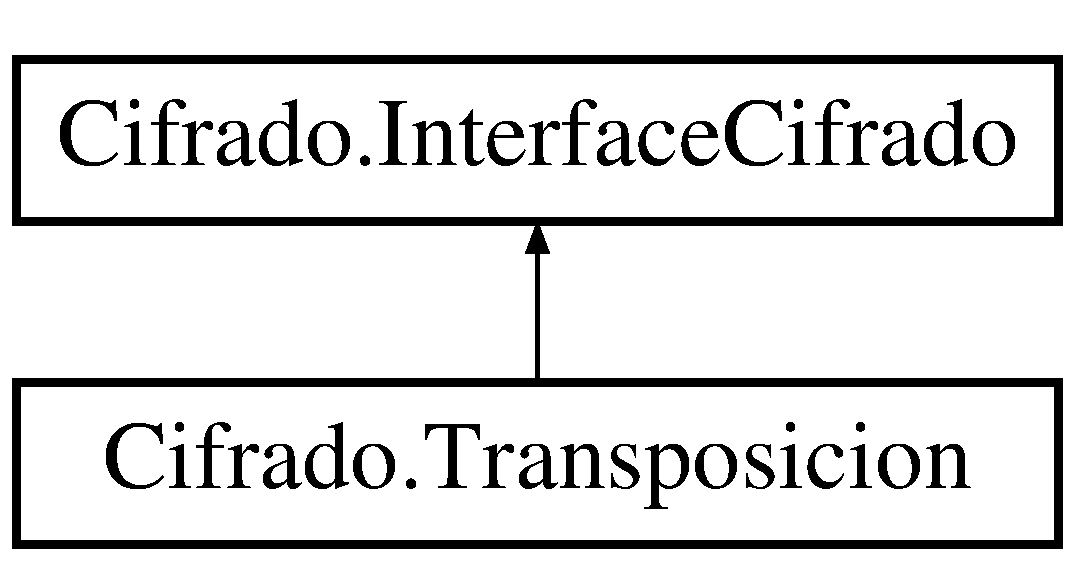
\includegraphics[height=2.000000cm]{interface_cifrado_1_1_interface_cifrado}
\end{center}
\end{figure}
\subsection*{Métodos públicos}
\begin{DoxyCompactItemize}
\item 
string \hyperlink{interface_cifrado_1_1_interface_cifrado_a67baf37475e65a3cf07a0546309cf391}{Cifrar} (string Input)
\begin{DoxyCompactList}\small\item\em Cifra un texto basado en una llave o metodo \end{DoxyCompactList}\item 
string \hyperlink{interface_cifrado_1_1_interface_cifrado_af7035203a5d4212ddcca039351dd3a22}{Descifrar} (string Input)
\begin{DoxyCompactList}\small\item\em Descifra un texto basado en una llave o metodo \end{DoxyCompactList}\item 
string \hyperlink{interface_cifrado_1_1_interface_cifrado_ade6b2a14d9cd48feec78c2695a2149bc}{Cifrar} ()
\begin{DoxyCompactList}\small\item\em Cifra un texto basado en una llave o metodo \end{DoxyCompactList}\item 
string \hyperlink{interface_cifrado_1_1_interface_cifrado_aef07884028ee90698a4a1202d851fecf}{Descifrar} ()
\begin{DoxyCompactList}\small\item\em Descifra un texto basado en una llave o metodo \end{DoxyCompactList}\item 
void \hyperlink{interface_cifrado_1_1_interface_cifrado_a0eee6d795ffd5d8f9971e1d8fb6f4b8d}{Getkey} (string Key)
\begin{DoxyCompactList}\small\item\em Actualiza la llave de cifrado \end{DoxyCompactList}\item 
void \hyperlink{interface_cifrado_1_1_interface_cifrado_ab573118c8f88269038b21e452a9fa8d3}{Get\+Input} (string Input)
\begin{DoxyCompactList}\small\item\em Actualiza el input de cada metodo \end{DoxyCompactList}\end{DoxyCompactItemize}


\subsection{Documentación de las funciones miembro}
\mbox{\Hypertarget{interface_cifrado_1_1_interface_cifrado_a67baf37475e65a3cf07a0546309cf391}\label{interface_cifrado_1_1_interface_cifrado_a67baf37475e65a3cf07a0546309cf391}} 
\index{Cifrado\+::\+Interface\+Cifrado@{Cifrado\+::\+Interface\+Cifrado}!Cifrar@{Cifrar}}
\index{Cifrar@{Cifrar}!Cifrado\+::\+Interface\+Cifrado@{Cifrado\+::\+Interface\+Cifrado}}
\subsubsection{\texorpdfstring{Cifrar()}{Cifrar()}\hspace{0.1cm}{\footnotesize\ttfamily [1/2]}}
{\footnotesize\ttfamily string Cifrado.\+Interface\+Cifrado.\+Cifrar (\begin{DoxyParamCaption}\item[{string}]{Input }\end{DoxyParamCaption})}



Cifra un texto basado en una llave o metodo 


\begin{DoxyParams}{Parámetros}
{\em Input} & parametro de entrada texto sin cifrar\\
\hline
\end{DoxyParams}
\begin{DoxyReturn}{Devuelve}
texto cifrado
\end{DoxyReturn}


Implementado en \hyperlink{class_cifrado_1_1_transposicion_a34feeb193fcf5f9bf3385043dae4b4c8}{Cifrado.\+Transposicion}.

\mbox{\Hypertarget{interface_cifrado_1_1_interface_cifrado_ade6b2a14d9cd48feec78c2695a2149bc}\label{interface_cifrado_1_1_interface_cifrado_ade6b2a14d9cd48feec78c2695a2149bc}} 
\index{Cifrado\+::\+Interface\+Cifrado@{Cifrado\+::\+Interface\+Cifrado}!Cifrar@{Cifrar}}
\index{Cifrar@{Cifrar}!Cifrado\+::\+Interface\+Cifrado@{Cifrado\+::\+Interface\+Cifrado}}
\subsubsection{\texorpdfstring{Cifrar()}{Cifrar()}\hspace{0.1cm}{\footnotesize\ttfamily [2/2]}}
{\footnotesize\ttfamily string Cifrado.\+Interface\+Cifrado.\+Cifrar (\begin{DoxyParamCaption}{ }\end{DoxyParamCaption})}



Cifra un texto basado en una llave o metodo 

\begin{DoxyReturn}{Devuelve}
texto cifrado
\end{DoxyReturn}


Implementado en \hyperlink{class_cifrado_1_1_transposicion_a3d6021ac06c306a6943e88c3678d97cf}{Cifrado.\+Transposicion}.

\mbox{\Hypertarget{interface_cifrado_1_1_interface_cifrado_af7035203a5d4212ddcca039351dd3a22}\label{interface_cifrado_1_1_interface_cifrado_af7035203a5d4212ddcca039351dd3a22}} 
\index{Cifrado\+::\+Interface\+Cifrado@{Cifrado\+::\+Interface\+Cifrado}!Descifrar@{Descifrar}}
\index{Descifrar@{Descifrar}!Cifrado\+::\+Interface\+Cifrado@{Cifrado\+::\+Interface\+Cifrado}}
\subsubsection{\texorpdfstring{Descifrar()}{Descifrar()}\hspace{0.1cm}{\footnotesize\ttfamily [1/2]}}
{\footnotesize\ttfamily string Cifrado.\+Interface\+Cifrado.\+Descifrar (\begin{DoxyParamCaption}\item[{string}]{Input }\end{DoxyParamCaption})}



Descifra un texto basado en una llave o metodo 


\begin{DoxyParams}{Parámetros}
{\em Input} & parametro de entrada texto cifrado\\
\hline
\end{DoxyParams}
\begin{DoxyReturn}{Devuelve}
texto descifrado
\end{DoxyReturn}


Implementado en \hyperlink{class_cifrado_1_1_transposicion_a45a8f6d97d2afdf5691c7197ae0187c4}{Cifrado.\+Transposicion}.

\mbox{\Hypertarget{interface_cifrado_1_1_interface_cifrado_aef07884028ee90698a4a1202d851fecf}\label{interface_cifrado_1_1_interface_cifrado_aef07884028ee90698a4a1202d851fecf}} 
\index{Cifrado\+::\+Interface\+Cifrado@{Cifrado\+::\+Interface\+Cifrado}!Descifrar@{Descifrar}}
\index{Descifrar@{Descifrar}!Cifrado\+::\+Interface\+Cifrado@{Cifrado\+::\+Interface\+Cifrado}}
\subsubsection{\texorpdfstring{Descifrar()}{Descifrar()}\hspace{0.1cm}{\footnotesize\ttfamily [2/2]}}
{\footnotesize\ttfamily string Cifrado.\+Interface\+Cifrado.\+Descifrar (\begin{DoxyParamCaption}{ }\end{DoxyParamCaption})}



Descifra un texto basado en una llave o metodo 

\begin{DoxyReturn}{Devuelve}
texto descifrado
\end{DoxyReturn}


Implementado en \hyperlink{class_cifrado_1_1_transposicion_ac2934aaba73bbaca8e5da6b788cf10b2}{Cifrado.\+Transposicion}.

\mbox{\Hypertarget{interface_cifrado_1_1_interface_cifrado_ab573118c8f88269038b21e452a9fa8d3}\label{interface_cifrado_1_1_interface_cifrado_ab573118c8f88269038b21e452a9fa8d3}} 
\index{Cifrado\+::\+Interface\+Cifrado@{Cifrado\+::\+Interface\+Cifrado}!Get\+Input@{Get\+Input}}
\index{Get\+Input@{Get\+Input}!Cifrado\+::\+Interface\+Cifrado@{Cifrado\+::\+Interface\+Cifrado}}
\subsubsection{\texorpdfstring{Get\+Input()}{GetInput()}}
{\footnotesize\ttfamily void Cifrado.\+Interface\+Cifrado.\+Get\+Input (\begin{DoxyParamCaption}\item[{string}]{Input }\end{DoxyParamCaption})}



Actualiza el input de cada metodo 


\begin{DoxyParams}{Parámetros}
{\em Input} & nuevo input para cada metodo\\
\hline
\end{DoxyParams}


Implementado en \hyperlink{class_cifrado_1_1_transposicion_a41f7391ffcd850e2aebf9852248d6d8d}{Cifrado.\+Transposicion}.

\mbox{\Hypertarget{interface_cifrado_1_1_interface_cifrado_a0eee6d795ffd5d8f9971e1d8fb6f4b8d}\label{interface_cifrado_1_1_interface_cifrado_a0eee6d795ffd5d8f9971e1d8fb6f4b8d}} 
\index{Cifrado\+::\+Interface\+Cifrado@{Cifrado\+::\+Interface\+Cifrado}!Getkey@{Getkey}}
\index{Getkey@{Getkey}!Cifrado\+::\+Interface\+Cifrado@{Cifrado\+::\+Interface\+Cifrado}}
\subsubsection{\texorpdfstring{Getkey()}{Getkey()}}
{\footnotesize\ttfamily void Cifrado.\+Interface\+Cifrado.\+Getkey (\begin{DoxyParamCaption}\item[{string}]{Key }\end{DoxyParamCaption})}



Actualiza la llave de cifrado 


\begin{DoxyParams}{Parámetros}
{\em Key} & nueva llave de cifrado\\
\hline
\end{DoxyParams}


Implementado en \hyperlink{class_cifrado_1_1_transposicion_ab35db490c8543ccb453b4384ad4e236c}{Cifrado.\+Transposicion}.



La documentación para este interfaz fue generada a partir del siguiente fichero\+:\begin{DoxyCompactItemize}
\item 
C\+:/\+Users/jaira/\+Documents/\+Visual Studio 2015/\+Projects/\+Cifrado\+Por\+Transposicion/\+Cifrado/Interface\+Cifrado.\+cs\end{DoxyCompactItemize}

\hypertarget{class_cifrado_1_1_transposicion}{}\section{Referencia de la Clase Cifrado.\+Transposicion}
\label{class_cifrado_1_1_transposicion}\index{Cifrado.\+Transposicion@{Cifrado.\+Transposicion}}


clase qeu hereda la interfaz \hyperlink{interface_cifrado_1_1_interface_cifrado}{Interface\+Cifrado} que contiene el funcionmiento basico de un metodo de cifrado  


Diagrama de herencias de Cifrado.\+Transposicion\begin{figure}[H]
\begin{center}
\leavevmode
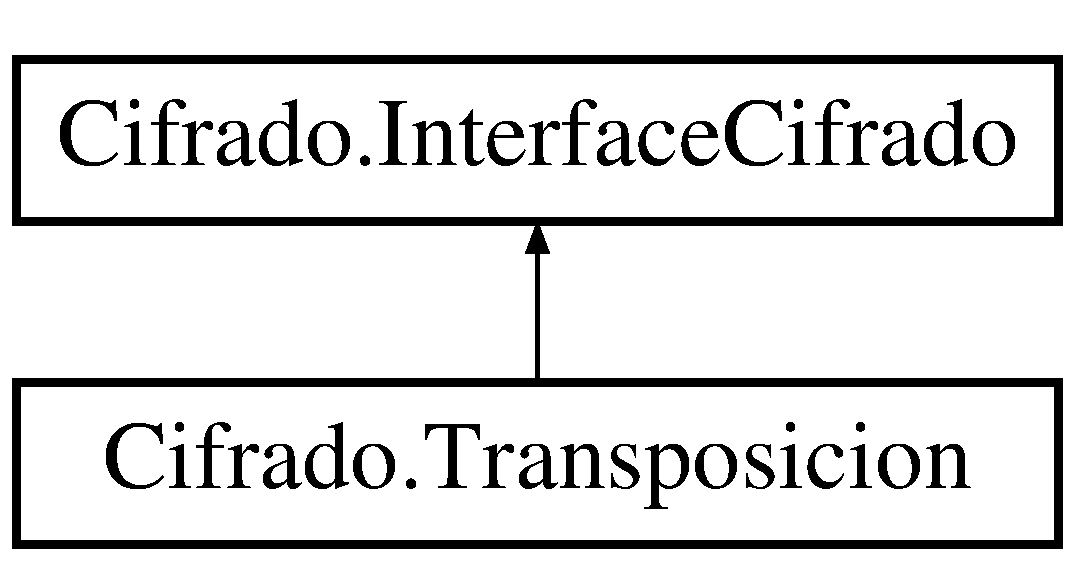
\includegraphics[height=2.000000cm]{class_cifrado_1_1_transposicion}
\end{center}
\end{figure}
\subsection*{Métodos públicos}
\begin{DoxyCompactItemize}
\item 
int \hyperlink{class_cifrado_1_1_transposicion_a8df16c3d60a6f57d8cf40b17a5f40925}{Dimenciones} (string \hyperlink{class_cifrado_1_1_transposicion_ae35952dd0b3f5c626fa4f7c084428f8a}{Input})
\begin{DoxyCompactList}\small\item\em permite calcular las dimenciones de una matriz cuadrada para un input \end{DoxyCompactList}\item 
string \hyperlink{class_cifrado_1_1_transposicion_a34feeb193fcf5f9bf3385043dae4b4c8}{Cifrar} (string \hyperlink{class_cifrado_1_1_transposicion_ae35952dd0b3f5c626fa4f7c084428f8a}{Input})
\begin{DoxyCompactList}\small\item\em Cifra un texto basado en una llave o metodo \end{DoxyCompactList}\item 
string \hyperlink{class_cifrado_1_1_transposicion_a3d6021ac06c306a6943e88c3678d97cf}{Cifrar} ()
\begin{DoxyCompactList}\small\item\em Cifra un texto basado en una llave o metodo \end{DoxyCompactList}\item 
string \hyperlink{class_cifrado_1_1_transposicion_a45a8f6d97d2afdf5691c7197ae0187c4}{Descifrar} (string \hyperlink{class_cifrado_1_1_transposicion_ae35952dd0b3f5c626fa4f7c084428f8a}{Input})
\begin{DoxyCompactList}\small\item\em Descifra un texto basado en una llave o metodo \end{DoxyCompactList}\item 
string \hyperlink{class_cifrado_1_1_transposicion_ac2934aaba73bbaca8e5da6b788cf10b2}{Descifrar} ()
\begin{DoxyCompactList}\small\item\em Descifra un texto basado en una llave o metodo \end{DoxyCompactList}\item 
void \hyperlink{class_cifrado_1_1_transposicion_ab35db490c8543ccb453b4384ad4e236c}{Getkey} (string \hyperlink{class_cifrado_1_1_transposicion_ada94313eb5cb29e6c95ade7bd2f8306f}{Key})
\begin{DoxyCompactList}\small\item\em Actualiza la llave de cifrado \end{DoxyCompactList}\item 
void \hyperlink{class_cifrado_1_1_transposicion_a41f7391ffcd850e2aebf9852248d6d8d}{Get\+Input} (string \hyperlink{class_cifrado_1_1_transposicion_ae35952dd0b3f5c626fa4f7c084428f8a}{Input})
\begin{DoxyCompactList}\small\item\em Actualiza el input de cada metodo \end{DoxyCompactList}\end{DoxyCompactItemize}
\subsection*{Propiedades}
\begin{DoxyCompactItemize}
\item 
int \hyperlink{class_cifrado_1_1_transposicion_a732e580b22860879283fd70933821194}{Length}\hspace{0.3cm}{\ttfamily  \mbox{[}get, set\mbox{]}}
\begin{DoxyCompactList}\small\item\em propiedad que permite modificar o recuperar la longitud del input a cifrar o descifrar \end{DoxyCompactList}\item 
string \hyperlink{class_cifrado_1_1_transposicion_ae35952dd0b3f5c626fa4f7c084428f8a}{Input}\hspace{0.3cm}{\ttfamily  \mbox{[}get, set\mbox{]}}
\begin{DoxyCompactList}\small\item\em propiedad que permite modificar o recuperar el input a cifrar o descifrar \end{DoxyCompactList}\item 
string \hyperlink{class_cifrado_1_1_transposicion_ada94313eb5cb29e6c95ade7bd2f8306f}{Key}\hspace{0.3cm}{\ttfamily  \mbox{[}get, set\mbox{]}}
\begin{DoxyCompactList}\small\item\em propiedad que permite modificar o recuperar la clave para cifrar o descifrar \end{DoxyCompactList}\item 
Data\+Table \hyperlink{class_cifrado_1_1_transposicion_a0befab6514e913da972697a59f27b14a}{Matriz}\hspace{0.3cm}{\ttfamily  \mbox{[}get, set\mbox{]}}
\begin{DoxyCompactList}\small\item\em propiedad que permite modificar o recuperar la matriz a trasponer \end{DoxyCompactList}\end{DoxyCompactItemize}


\subsection{Descripción detallada}
clase qeu hereda la interfaz \hyperlink{interface_cifrado_1_1_interface_cifrado}{Interface\+Cifrado} que contiene el funcionmiento basico de un metodo de cifrado 



\subsection{Documentación de las funciones miembro}
\mbox{\Hypertarget{class_cifrado_1_1_transposicion_a34feeb193fcf5f9bf3385043dae4b4c8}\label{class_cifrado_1_1_transposicion_a34feeb193fcf5f9bf3385043dae4b4c8}} 
\index{Cifrado\+::\+Transposicion@{Cifrado\+::\+Transposicion}!Cifrar@{Cifrar}}
\index{Cifrar@{Cifrar}!Cifrado\+::\+Transposicion@{Cifrado\+::\+Transposicion}}
\subsubsection{\texorpdfstring{Cifrar()}{Cifrar()}\hspace{0.1cm}{\footnotesize\ttfamily [1/2]}}
{\footnotesize\ttfamily string Cifrado.\+Transposicion.\+Cifrar (\begin{DoxyParamCaption}\item[{string}]{Input }\end{DoxyParamCaption})}



Cifra un texto basado en una llave o metodo 


\begin{DoxyParams}{Parámetros}
{\em Input} & parametro de entrada texto sin cifrar\\
\hline
\end{DoxyParams}
\begin{DoxyReturn}{Devuelve}
texto cifrado
\end{DoxyReturn}


Implementa \hyperlink{interface_cifrado_1_1_interface_cifrado_a67baf37475e65a3cf07a0546309cf391}{Cifrado.\+Interface\+Cifrado}.

\mbox{\Hypertarget{class_cifrado_1_1_transposicion_a3d6021ac06c306a6943e88c3678d97cf}\label{class_cifrado_1_1_transposicion_a3d6021ac06c306a6943e88c3678d97cf}} 
\index{Cifrado\+::\+Transposicion@{Cifrado\+::\+Transposicion}!Cifrar@{Cifrar}}
\index{Cifrar@{Cifrar}!Cifrado\+::\+Transposicion@{Cifrado\+::\+Transposicion}}
\subsubsection{\texorpdfstring{Cifrar()}{Cifrar()}\hspace{0.1cm}{\footnotesize\ttfamily [2/2]}}
{\footnotesize\ttfamily string Cifrado.\+Transposicion.\+Cifrar (\begin{DoxyParamCaption}{ }\end{DoxyParamCaption})}



Cifra un texto basado en una llave o metodo 

\begin{DoxyReturn}{Devuelve}
texto cifrado
\end{DoxyReturn}


Implementa \hyperlink{interface_cifrado_1_1_interface_cifrado_ade6b2a14d9cd48feec78c2695a2149bc}{Cifrado.\+Interface\+Cifrado}.

\mbox{\Hypertarget{class_cifrado_1_1_transposicion_a45a8f6d97d2afdf5691c7197ae0187c4}\label{class_cifrado_1_1_transposicion_a45a8f6d97d2afdf5691c7197ae0187c4}} 
\index{Cifrado\+::\+Transposicion@{Cifrado\+::\+Transposicion}!Descifrar@{Descifrar}}
\index{Descifrar@{Descifrar}!Cifrado\+::\+Transposicion@{Cifrado\+::\+Transposicion}}
\subsubsection{\texorpdfstring{Descifrar()}{Descifrar()}\hspace{0.1cm}{\footnotesize\ttfamily [1/2]}}
{\footnotesize\ttfamily string Cifrado.\+Transposicion.\+Descifrar (\begin{DoxyParamCaption}\item[{string}]{Input }\end{DoxyParamCaption})}



Descifra un texto basado en una llave o metodo 


\begin{DoxyParams}{Parámetros}
{\em Input} & parametro de entrada texto cifrado\\
\hline
\end{DoxyParams}
\begin{DoxyReturn}{Devuelve}
texto descifrado
\end{DoxyReturn}


Implementa \hyperlink{interface_cifrado_1_1_interface_cifrado_af7035203a5d4212ddcca039351dd3a22}{Cifrado.\+Interface\+Cifrado}.

\mbox{\Hypertarget{class_cifrado_1_1_transposicion_ac2934aaba73bbaca8e5da6b788cf10b2}\label{class_cifrado_1_1_transposicion_ac2934aaba73bbaca8e5da6b788cf10b2}} 
\index{Cifrado\+::\+Transposicion@{Cifrado\+::\+Transposicion}!Descifrar@{Descifrar}}
\index{Descifrar@{Descifrar}!Cifrado\+::\+Transposicion@{Cifrado\+::\+Transposicion}}
\subsubsection{\texorpdfstring{Descifrar()}{Descifrar()}\hspace{0.1cm}{\footnotesize\ttfamily [2/2]}}
{\footnotesize\ttfamily string Cifrado.\+Transposicion.\+Descifrar (\begin{DoxyParamCaption}{ }\end{DoxyParamCaption})}



Descifra un texto basado en una llave o metodo 

\begin{DoxyReturn}{Devuelve}
texto descifrado
\end{DoxyReturn}


Implementa \hyperlink{interface_cifrado_1_1_interface_cifrado_aef07884028ee90698a4a1202d851fecf}{Cifrado.\+Interface\+Cifrado}.

\mbox{\Hypertarget{class_cifrado_1_1_transposicion_a8df16c3d60a6f57d8cf40b17a5f40925}\label{class_cifrado_1_1_transposicion_a8df16c3d60a6f57d8cf40b17a5f40925}} 
\index{Cifrado\+::\+Transposicion@{Cifrado\+::\+Transposicion}!Dimenciones@{Dimenciones}}
\index{Dimenciones@{Dimenciones}!Cifrado\+::\+Transposicion@{Cifrado\+::\+Transposicion}}
\subsubsection{\texorpdfstring{Dimenciones()}{Dimenciones()}}
{\footnotesize\ttfamily int Cifrado.\+Transposicion.\+Dimenciones (\begin{DoxyParamCaption}\item[{string}]{Input }\end{DoxyParamCaption})}



permite calcular las dimenciones de una matriz cuadrada para un input 


\begin{DoxyParams}{Parámetros}
{\em Input} & cadena de texto plano\\
\hline
\end{DoxyParams}
\begin{DoxyReturn}{Devuelve}
la dimencion de la matriz cuadrada que puede almacenar el input
\end{DoxyReturn}
\mbox{\Hypertarget{class_cifrado_1_1_transposicion_a41f7391ffcd850e2aebf9852248d6d8d}\label{class_cifrado_1_1_transposicion_a41f7391ffcd850e2aebf9852248d6d8d}} 
\index{Cifrado\+::\+Transposicion@{Cifrado\+::\+Transposicion}!Get\+Input@{Get\+Input}}
\index{Get\+Input@{Get\+Input}!Cifrado\+::\+Transposicion@{Cifrado\+::\+Transposicion}}
\subsubsection{\texorpdfstring{Get\+Input()}{GetInput()}}
{\footnotesize\ttfamily void Cifrado.\+Transposicion.\+Get\+Input (\begin{DoxyParamCaption}\item[{string}]{Input }\end{DoxyParamCaption})}



Actualiza el input de cada metodo 


\begin{DoxyParams}{Parámetros}
{\em Input} & nuevo input para cada metodo\\
\hline
\end{DoxyParams}


Implementa \hyperlink{interface_cifrado_1_1_interface_cifrado_ab573118c8f88269038b21e452a9fa8d3}{Cifrado.\+Interface\+Cifrado}.

\mbox{\Hypertarget{class_cifrado_1_1_transposicion_ab35db490c8543ccb453b4384ad4e236c}\label{class_cifrado_1_1_transposicion_ab35db490c8543ccb453b4384ad4e236c}} 
\index{Cifrado\+::\+Transposicion@{Cifrado\+::\+Transposicion}!Getkey@{Getkey}}
\index{Getkey@{Getkey}!Cifrado\+::\+Transposicion@{Cifrado\+::\+Transposicion}}
\subsubsection{\texorpdfstring{Getkey()}{Getkey()}}
{\footnotesize\ttfamily void Cifrado.\+Transposicion.\+Getkey (\begin{DoxyParamCaption}\item[{string}]{Key }\end{DoxyParamCaption})}



Actualiza la llave de cifrado 


\begin{DoxyParams}{Parámetros}
{\em Key} & nueva llave de cifrado\\
\hline
\end{DoxyParams}


Implementa \hyperlink{interface_cifrado_1_1_interface_cifrado_a0eee6d795ffd5d8f9971e1d8fb6f4b8d}{Cifrado.\+Interface\+Cifrado}.



\subsection{Documentación de propiedades}
\mbox{\Hypertarget{class_cifrado_1_1_transposicion_ae35952dd0b3f5c626fa4f7c084428f8a}\label{class_cifrado_1_1_transposicion_ae35952dd0b3f5c626fa4f7c084428f8a}} 
\index{Cifrado\+::\+Transposicion@{Cifrado\+::\+Transposicion}!Input@{Input}}
\index{Input@{Input}!Cifrado\+::\+Transposicion@{Cifrado\+::\+Transposicion}}
\subsubsection{\texorpdfstring{Input}{Input}}
{\footnotesize\ttfamily string Cifrado.\+Transposicion.\+Input\hspace{0.3cm}{\ttfamily [get]}, {\ttfamily [set]}}



propiedad que permite modificar o recuperar el input a cifrar o descifrar 

\mbox{\Hypertarget{class_cifrado_1_1_transposicion_ada94313eb5cb29e6c95ade7bd2f8306f}\label{class_cifrado_1_1_transposicion_ada94313eb5cb29e6c95ade7bd2f8306f}} 
\index{Cifrado\+::\+Transposicion@{Cifrado\+::\+Transposicion}!Key@{Key}}
\index{Key@{Key}!Cifrado\+::\+Transposicion@{Cifrado\+::\+Transposicion}}
\subsubsection{\texorpdfstring{Key}{Key}}
{\footnotesize\ttfamily string Cifrado.\+Transposicion.\+Key\hspace{0.3cm}{\ttfamily [get]}, {\ttfamily [set]}}



propiedad que permite modificar o recuperar la clave para cifrar o descifrar 

\mbox{\Hypertarget{class_cifrado_1_1_transposicion_a732e580b22860879283fd70933821194}\label{class_cifrado_1_1_transposicion_a732e580b22860879283fd70933821194}} 
\index{Cifrado\+::\+Transposicion@{Cifrado\+::\+Transposicion}!Length@{Length}}
\index{Length@{Length}!Cifrado\+::\+Transposicion@{Cifrado\+::\+Transposicion}}
\subsubsection{\texorpdfstring{Length}{Length}}
{\footnotesize\ttfamily int Cifrado.\+Transposicion.\+Length\hspace{0.3cm}{\ttfamily [get]}, {\ttfamily [set]}}



propiedad que permite modificar o recuperar la longitud del input a cifrar o descifrar 

\mbox{\Hypertarget{class_cifrado_1_1_transposicion_a0befab6514e913da972697a59f27b14a}\label{class_cifrado_1_1_transposicion_a0befab6514e913da972697a59f27b14a}} 
\index{Cifrado\+::\+Transposicion@{Cifrado\+::\+Transposicion}!Matriz@{Matriz}}
\index{Matriz@{Matriz}!Cifrado\+::\+Transposicion@{Cifrado\+::\+Transposicion}}
\subsubsection{\texorpdfstring{Matriz}{Matriz}}
{\footnotesize\ttfamily Data\+Table Cifrado.\+Transposicion.\+Matriz\hspace{0.3cm}{\ttfamily [get]}, {\ttfamily [set]}}



propiedad que permite modificar o recuperar la matriz a trasponer 



La documentación para esta clase fue generada a partir del siguiente fichero\+:\begin{DoxyCompactItemize}
\item 
C\+:/\+Users/jaira/\+Documents/\+Visual Studio 2015/\+Projects/\+Cifrado\+Por\+Transposicion/\+Cifrado/Transposicion.\+cs\end{DoxyCompactItemize}

%--- End generated contents ---

% Index
\backmatter
\newpage
\phantomsection
\clearemptydoublepage
\addcontentsline{toc}{chapter}{Índice}
\printindex

\end{document}
